The brain has evolved to shape behaviour based on a lifetime of interaction,
learning and memory.  By contrast—and historically, of necessity—our
understanding of brain function has mostly derived from short-duration
controlled experiments.  While such experiments reveal key functional building
blocks, they cannot explore the full gamut of ethology; nor tell us how the
blocks fit together to shape lifelong behaviour.

Recent advances in recording, video, and signal-processing technology make
possible naturalistic, long-duration and continual (NaLoDuCo) experiments.  The
partners in this proposal have pioneered this transition. The
Aeon platform~\citep{campagnerEtAl25b} developed at the Sainsbury Wellcome Centre (SWC) and Gatsby
Unit with support from NeuroGEARS, and adapted by the Allen Institute for
Neural Dynamics (AIND), provides a modular environment of mechatronic elements
and monitoring and recording pathways, enabling continuous high-resolution
behavioural and neural measurement over an unprecedented timescale of many
weeks to months (Figure). Aeon enables a new type of neuroscience experiment.
Rather than tightly controlled, isolated, trial-based stimulus-behaviour
contingencies, multiple contingencies are embedded in a single environment that
animals explore, learn about, and engage with over weeks. Examples include mice
foraging from patches of varying difficulty and rates of success
\citep[SWC/Gatsby;][]{campagnerEtAl25b} and the gradual acquisition of naturalistic olfactory
associations \citep[AIND;][]{finkEtAl24}. Continual high-resolution video and neurophysiological
recording expose the neural underpinnings of all phases of these behaviours:
including self-paced decisions about engagement with elements of the
environment, internally-directed exploration, sensorimotor control within each
local patch, memory and replay events during engagement and during sleep, and
more.

Central to Aeon is the vision of open science. The design specifications of the
system and components are shared openly\footnote{https://aeon.swc.ucl.ac.uk}.
Data collection is performed with the open-source Bonsai software
ecosystem~\citep{lopesEtAl15} supported by NeuroGEARS. Critical is that data
collected within Aeon be made available rapidly and easily to scientists
worldwide, providing a rich, expanding and coherent data resource that will
accelerate discovery.

While naturalistic, long-duration, or continuous neuroscience experiments have
been conducted in the past
\citep{nagyEtAl23,hoEtAl23,rayEtAl25,weissbrodEtAl13,dhawaleEtAl17,newmanEtAl25},
to the best of our knowledge, we are the first ones to integrate all three of
these features in a single experimental paradigm.
%
% Experiments of this type have been advocated by experts in the field years
% ago \citep[][p19]{dattaEtAl19}, yet they have not been implemented so far.

% \subsubsection{Neural data analysis at scale}

The pivotal lesson from AI is that data scale and diversity unlock model
capacity. ImageNet supplied enough variation for deep networks to discover
general features that smaller corpora could never support. NaLoDuCo recordings
aim to do the same for neuroscience.
%
The scale of NaLoDuCo datasets enables questions—and models—that short datasets
cannot:

\begin{description}

	\item[Temporal depth:] Learn representations over hours-to-weeks, capturing
slow plasticity, representational drift, consolidation, and circadian cycles.

	\item[Rare phenomena:] Detect and model low-frequency events
(reorientations, replay, state transitions) that are under-sampled in standard
datasets.

	\item[Context richness:] Jointly model neural activity with behavior,
environment, and internal state (sleep, arousal), allowing multimodal,
self-supervised objectives that need long contexts.

	\item[Generalization:] Train foundation-style models that transfer across
animals, days, and tasks—something infeasible with small, episodic data.

	\item[Closed-loop readiness:] Train low-latency decoders and predictive
controllers that remain reliable across the full spectrum of natural
variability—a robustness that only emerges with long-duration data.

\end{description}

NaLoDuCo’s scale allow powerful models to see the brain at the timescales where
its organizing principles live—just as large-scale datasets did for deep
learning in computer vision.

This emerging paradigm of long-duration experimentation is poised to become
mainstream in the coming years.
%
However, experiments spanning weeks to months generate massive datasets—often
reaching hundreds of terabytes—posing significant challenges in data
acquisition, management, distribution, visualisation, and analysis.
%
To address these challenges, we (GCNU, SWC, AIND, and NeuroGEARS Ltd) will
collaboratively extend the AEON platform with functionality to share,
visualise and statistically analyse NaLoDuCo experimental data where it
leaves, in the cloud or in institutional clusters.

\subsubsection{Specific aims}

\begin{description}

    \item[Data sharing:] Data generated by NaLoDuCo experiments will be of general interest to the
neuroscience community. We want to share our NaLoDuCo foraging and odour
learning recordings and allow other groups collecting this type of data to
share their own, and to allow users interested in accessing our data to do so,
for example, to analyze our NaLoDuCo recordings with new artificial
intelligence algorithms.

A milestone in AI happened in 2010 when deep neural network models achieved unprecedented performance in computer vision tasks. This performance boost critically depended on the existence of the MNIST dataset, without which AI would not be what it is today. We envision that NaLoDuCo datasets will mean for the neuroscience community what MNIST meant to the computer vision one.

%
However, this dissemination is not trivial, as datasets are of the order of
hundreds of terabytes, and it will take users several days to download them
over standard Internet connections.

Instead of bringing data to users, we will bring users to data, by storing
datasets in the cloud, or in institutional high-performance-computing (HPC)
systems, and providing \textbf{cloud software to allow users to visually
explore and statistically analyse behavioural and neural NaLoDuCo datasets
where they live} (1 and 2 in Figure~\ref{fig:aims}).

Our statistical analysis of neural time series will require knowledge of the
spiking activity of single units; i.e., spike sorting. In long-duration
experiments with freely moving animals spike sorting is a challenging problem,
because movements of recording probes change the shape of spike waveforms over
time and complicate the assignment of spikes to units based on their waveforms.
We will address this problem by developing \textbf{spike sorting methods for
long-duration, continual and high-channel-count recordings} (3 in
Figure~\ref{fig:aims}).

Funded by a BBSRC award we are adding machine learning functionality to Bonsai
in order to enable a new type of experimentation controlled by advanced machine
learning inference on behavioural and neural
recordings~\citep[Bonsai.ML,][]{guilbeaultEtAl25}. We have developed this
functionality for conventional short duration experiments. We will add to
Bonsai.ML \textbf{real-time machine learning functionality for processing
nonstationary data}, such as that generated in NaLoDuCo experiments.

Most of the online neural data analysis methods that we will add to AEON
require sorted spikes. We will adapt the previous offline \textbf{spike sorting
methods for long-duration experiment to operate in real-time} (5 in
Figure~\ref{fig:aims}).

\end{description}

\begin{figure}
    \begin{center}
        % 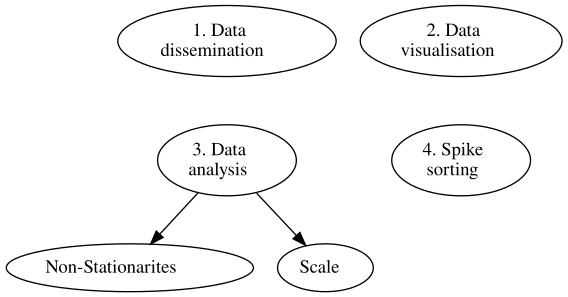
\includegraphics[width=3in]{figures/aims.png}
    \end{center}
    \caption{Specific aims}
    \label{fig:aims}
\end{figure}

Our goal is to fully realise this vision, by developing complementary platform
technologies for data analysis, visualisation and sharing.
We will build core signal-processing and modelling pathways, and an integrated
platform to visualise and analyse remote-host-based data.

To do so, we must overcome challenges raised by the scale and structure of
NaLoDuCo experiments. Analyses must track non-stationarity in underlying
signals (including in the identification of action potentials from separate
neurons). Data volumes (potentially reaching hundreds of terabytes) preclude
simple sharing. Instead we will develop a remote-based framework allowing users
to explore and analyse behavioural and neural datasets in situ; with data
uploaded once but used repeatedly.
